\resizebox{5cm}{!}{
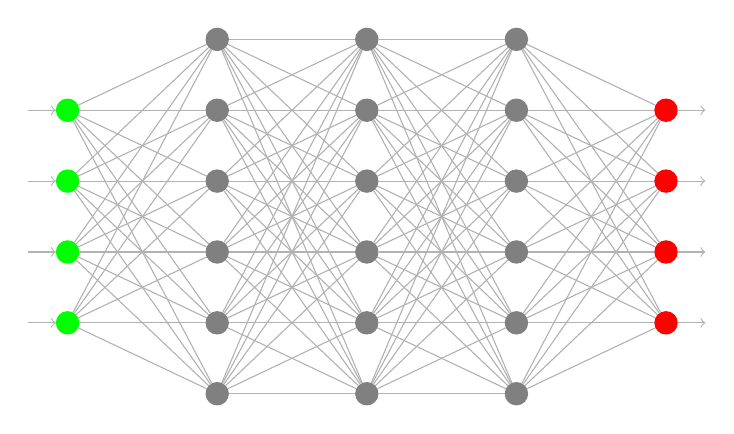
\begin{tikzpicture}[node distance=0.9cm,
	font=\scriptsize,auto,
	every node/.style={circle,inner sep=0.1cm},
	input/.style={fill=green,draw=green},
	hidden/.style={fill=black!50!white,draw=black!50!white},
	output/.style={fill=red,draw=red}]

  
  \node [input] (i1) {};
  \node [below of=i1, input] (i2) {};
  \node [below of=i2, input] (i3) {};
  \node [below of=i3, input] (i4) {};

  \node [right of = i1, above of = i1, xshift=1cm, hidden] (h11) {};
  \node [below of=h11, hidden] (h12) {};
  \node [below of=h12, hidden] (h13) {};
  \node [below of=h13, hidden] (h14) {};
  \node [below of=h14, hidden] (h15) {};
  \node [below of=h15, hidden] (h16) {};

  \node [right of = h11, xshift=1cm, hidden] (h21) {};
  \node [below of=h21, hidden] (h22) {};
  \node [below of=h22, hidden] (h23) {};
  \node [below of=h23, hidden] (h24) {};
  \node [below of=h24, hidden] (h25) {};
  \node [below of=h25, hidden] (h26) {};

  \node [right of = h21, xshift=1cm, hidden] (h31) {};
  \node [below of=h31, hidden] (h32) {};
  \node [below of=h32, hidden] (h33) {};
  \node [below of=h33, hidden] (h34) {};
  \node [below of=h34, hidden] (h35) {};
  \node [below of=h35, hidden] (h36) {};

  \node [right of = h32, xshift=1cm, output] (o1) {};
  \node [below of=o1, output] (o2) {};
  \node [below of=o2, output] (o3) {};
  \node [below of=o3, output] (o4) {};
  %\node [right of=1, xshift=-1.52m, fill=gray!50!white,draw=gray,neuron] (3) {};

  \foreach \i in {1,...,4}{
	  \draw[<-,color=black!30!white] (i\i) -- ++(-0.5,0);
	  \draw[->,color=black!30!white] (o\i) -- ++(0.5,0);
  }
  \foreach \i in {1,...,4}{
	 \foreach \j in {1,...,6}{
		 \draw [color=black!30!white]  (i\i) -- (h1\j);
   }}
  \foreach \i in {1,...,6}{
	 \foreach \j in {1,...,6}{
		 \draw [color=black!30!white]  (h1\i) -- (h2\j);
		 \draw [color=black!30!white]  (h2\i) -- (h3\j);
   }}
  \foreach \i in {1,...,6}{
	 \foreach \j in {1,...,4}{
		 \draw [color=black!30!white]  (h3\i) -- (o\j);
   }}

   %\node[below of=h16,xshift=-1cm,yshift=-0.5cm,input,label=right:{input node}] (inf1) {};
   %\node[right of=inf1,xshift=1.5cm,hidden,label=right:{hidden node}] (inf2) {};
   %\node[right of=inf2,xshift=1.5cm,output,label=right:{output node}] (inf3) {};

\end{tikzpicture}
}
